\Exhibit{VedomostiWikipedia}{%
    Статья в Wikipedia о газете Ведомости%
}

Это скриншот статьи в Wikipedia о газете Ведомости. В ней говорится:

\begin{itemize}

    \item Это бизнес-газета.

    \item Тираж больше 64000 экземпляров.

    \item \Quote{Ведомости основаны в 1999 году как совместное предприятие Dow Jones,
    который публикует \ul{The Wall Street Journal}; Pearson, который раньше публиковал \ul{Financial Times};
    и Independent Media, которые публикуют The Moscow Times.}

\end{itemize}

Это подтверждает значимость газеты и позволяет цитировать доход Calltouch, указанный в ней.

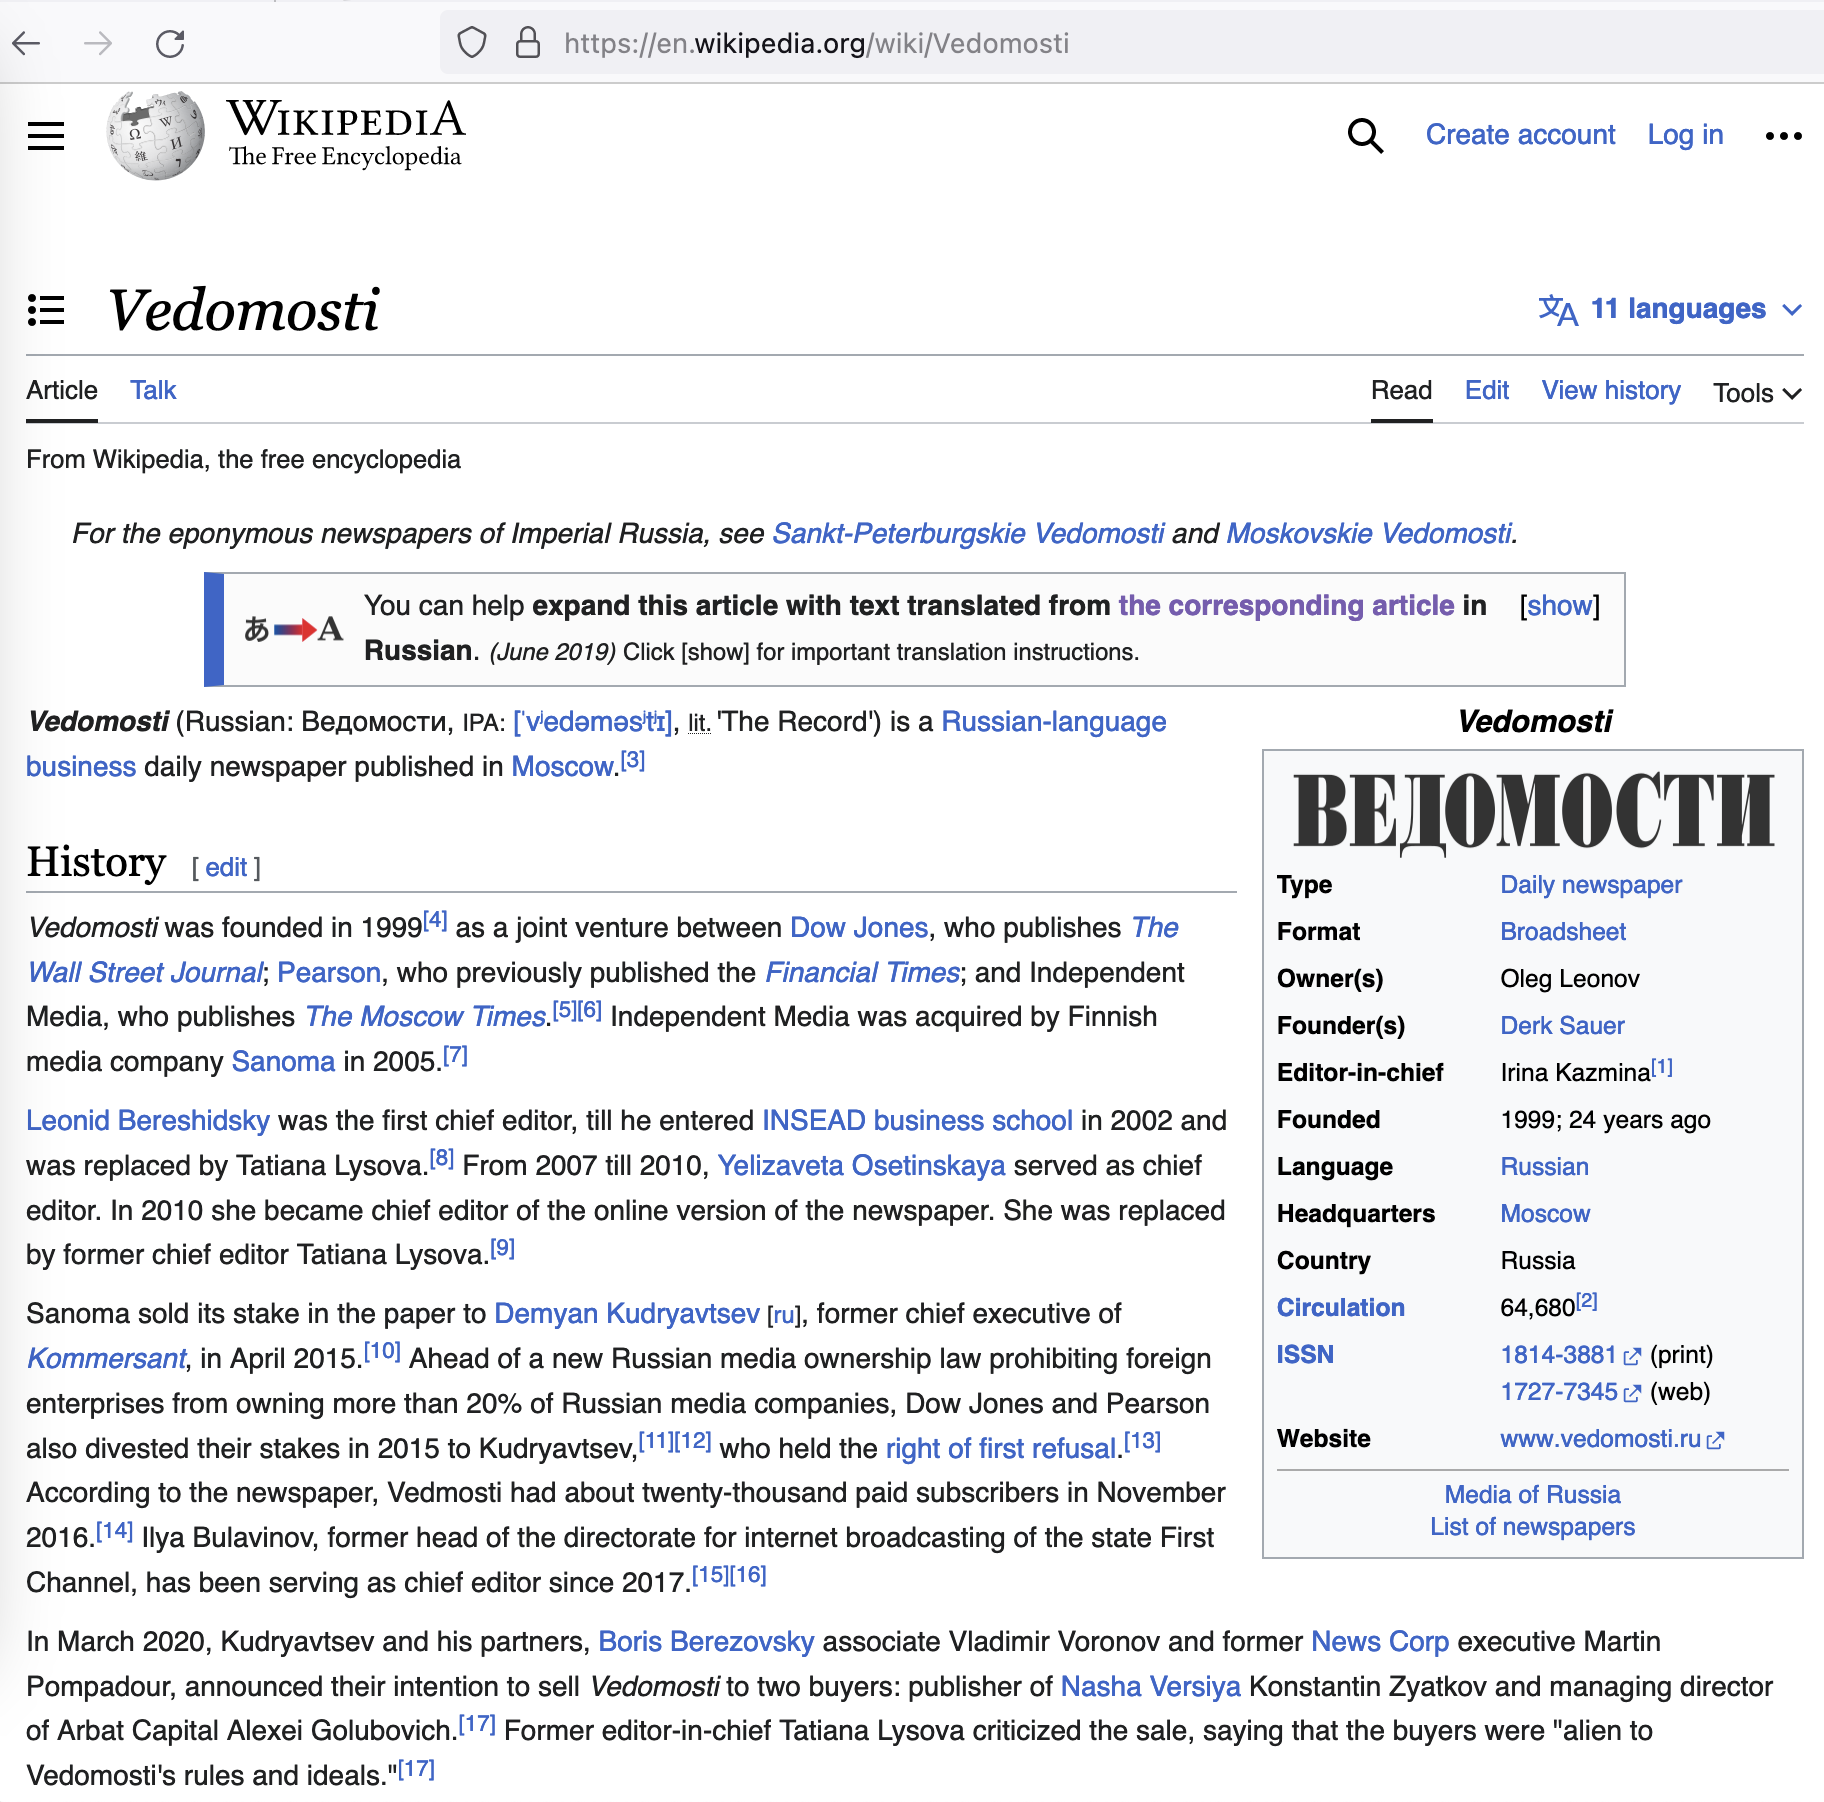
\includegraphics[width=\textwidth]{wikipedia-vedomosti}

\pagebreak
